% !TeX spellcheck = en_GB

\documentclass[aspectratio=169,]{beamer}

\usepackage[utf8]{inputenc}
\usepackage[english]{babel}
%\usepackage{appendixnumberbeamer}

\usepackage{tikz}
\usetikzlibrary{shapes,arrows,positioning,calc}

\tikzstyle{startstop} = [ellipse, draw, fill=bg, text=structure, text width=3em, text badly centered, inner sep=0pt]
\tikzstyle{block} = [rectangle, draw, fill=bg, text=structure, text width=5em, text centered]
\tikzstyle{decision} = [diamond, aspect=3, draw, fill=bg, text=structure, text width=3em, text badly centered, inner sep=0pt]
\tikzstyle{input} = [trapezium, draw, fill=bg, text=structure, text width=5em, text centered, trapezium right angle=120]
\tikzstyle{output} = [trapezium, draw, fill=bg, text=structure, text width=5em, text centered, trapezium right angle=120]

\tikzstyle{line} = [draw, -latex']

%\usepackage{xcolor}
\usepackage{listings}

\lstdefinestyle{pseudo}{
	backgroundcolor=\color{bg},
	keywordstyle=\color{alert},
	numberstyle=\tiny\color{fg!50},
	numbers=left,
	%commentstyle=\color{mGreen},
	%stringstyle=\color{mPurple},
    mathescape=true,
	basicstyle=\scriptsize,
    keywords={input,output,begin,end,if,then,else,while,do,for,each,return}
	%tabsize=4,
	%breakatwhitespace=false,
	%breaklines=true,
	%captionpos=b,
	%keepspaces=true,
	%numbersep=5pt,
	%showspaces=false,
	%showstringspaces=false,
	%showtabs=false,
	%language=C
}

\usepackage{minted}


\usetheme[titleformat=smallcaps, numbering=fraction, background=light, progressbar=frametitle]{metropolis}

\title{Digital Technology}
\subtitle{NumPy}

\author{Stefano Cereda\\
stefano.cereda@polimi.it
}
\date{28/04/2020}
\institute[PoliMi]{Politecnico Milano}
\logo{
\includegraphics[width=15mm]{../logopolimi}}

\setbeamercovered{invisible}

\makeindex

\begin{document}
\begin{frame}
    \maketitle
\end{frame}

\begin{frame}[fragile]{NumPy}
    NumPy\footnote{\url{https://numpy.org/}} is the fundamental package for scientific computing with Python. It contains among other things:
    \begin{itemize}
        \item a powerful N-dimensional array object
        \item sophisticated (broadcasting) functions
        \item tools for integrating C/C++ and Fortran code
        \item useful linear algebra, Fourier transform, and random number capabilities
    \end{itemize}

    %Allowing:
    %\begin{itemize}
    %    \item memory efficient, contiguous array
    %    \item easy and fast linear algebra operations
    %    \item more complex libraries (e.g., pandas)
    %\end{itemize}

    \centering
    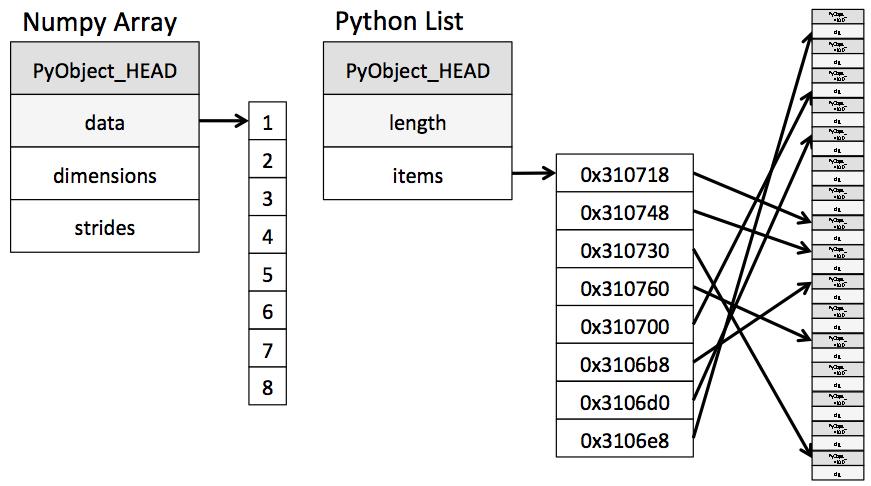
\includegraphics[width=.4\textwidth]{./memory.png}
\end{frame}

\begin{frame}[fragile, allowframebreaks]{NumPy Array}
    The main object offered by NumPy is the \emph{homogeneous multidimensional array}.
    It is a table of elements (all of the same type) indexed by a tuple of non-negative integers.

    We can easily convert a Python list to a NumPy array:
    \begin{minted}[autogobble,fontsize=\small]{Python}
        import numpy as np
        l = [1,2,3,4]
        a = np.array(l)
        print(a)
        print(a.ndim)  # number of dimensions (or axes)
        print(a.shape)  # the dimensions
        print(a.dtype)  # the data type of the array
    \end{minted}
    \framebreak

    Starting from a list of lists, we can create a 2D array:
    \begin{minted}[autogobble]{Python}
        # 2D array
        l = [[1,2,3], [10,20,30]]
        a = np.array(l)
        print(a)
        print(a.ndim)  # number of dimensions (or axes)
        print(a.shape)  # the dimensions
        print(a.dtype)  # the data type of the array
    \end{minted}
\end{frame}

\begin{frame}[fragile]{Array Creation --- Data Type}
    When creating an array from an iterable sequence, you can also specify the data type:
    \begin{minted}[autogobble]{Python}
    np.array([1,0,1,0], dtype=np.bool)
    np.array([1,0,1,0], dtype=np.int8)
    np.array([1,0,1,0], dtype=np.float64)
    \end{minted}
\end{frame}

\begin{frame}[fragile]{Array Creation --- Other Functions}
    Usually, we do not have a list with the interesting values, but we know the final dimension of our array. We can
    thus create arrays with initial placeholder content, minimizing the necessity of growing arrays, an expensive
    operation.
    \begin{minted}[autogobble, fontsize=\small]{Python}
        np.ones((3,4))  # a 2D 3x4 array full of ones
        np.zeros((2,3,3,4), dtype=np.int8)  # a 3D 2x3x4 full of zeros
        np.empty(10)  # a non-initialized one dimensional array

        np.arange(10, 30, 5)  # equivalent to np.array(range(10, 30, 5))
        np.linspace(0, 2*np.pi, 100)  # an array of 100 numbers from 0 to 2π
    \end{minted}

    The default data type is float64
\end{frame}

\begin{frame}[fragile,allowframebreaks]{Basic Operations}
    Arithmetic operators on arrays apply \emph{elemetwise}.
    A \emph{new} array is created and filled with the result:
    \begin{minted}[autogobble, fontsize=\small]{Python}
        a = np.array([1,2,3,4])
        b = np.array([1,2,1,2])
        print(a + b)
        print(a - b)
        print(a * b)
        print(a / b)
        print(a ** b)
        print(a > b)
    \end{minted}

    \framebreak
    The matrix product can be performed with the \texttt{@} operator or the \texttt{.dot} function or method:
    \begin{minted}[autogobble, fontsize=\small]{Python}
        a@b
        a.dot(b)
        np.dot(a, b)
    \end{minted}
\end{frame}

\begin{frame}[fragile,allowframebreaks]{Universal functions}
    NumPy provides common mathematical functions that operate elementwise on an array and produce an array as result,
    such as:
    \texttt{sin, cos, exp, all, any, argmax, argmin, argsort, average, ceil, clip, cumprod, cumsum, floor, invert, max,
    mean, median, min, minimum, round, sort, std, sum, trace, transpose} and many others.

    \framebreak
    Most of them support an axis argument, specifying the axis or axes (dimensions) along which to compute the function:
    \begin{minted}[autogobble, fontsize=\small]{Python}
        a = np.array([[1,2,3,4], [3,4,5,6]])
        np.mean(a)  # default is on flattened array
        np.mean(a, axis=0)  # average over first dimension
        np.mean(a, axis=1)  # average over second dimension
        np.mean(a, axis=(0,1))  # average over both dimensions
    \end{minted}
\end{frame}



\begin{frame}[fragile, allowframebreaks]{Indexing, Slicing and Iterating}
    One-dimensional arrays can be indexed, sliced and iterated over just like lists and other Python sequences:
    \begin{minted}[autogobble, fontsize=\small]{Python}
        a = np.arange(10)
        a[2]
        a[2:5]
        a[:6:2] = 1000
    \end{minted}

    \framebreak
    Multidimensional arrays can have one index per axis, given in a tuple:
    \begin{minted}[autogobble, fontsize=\small]{Python}
        def f(x, y):
            return 10*x + y

        a = np.fromfunction(f, (5,4), dtype=int)
        print(a)

        a[2,3]  # 23
        a[0:5, 1]  # row from 0 to 4 (all), first column
        a[:, 1]  # all rows, first column
        a[-1]  # last row, equivalent to a[-1, :]
    \end{minted}

    \framebreak
    Iteration is done from first axis:
    \begin{minted}[autogobble, fontsize=\small]{Python}
        matrix = np.fromfunction(f, (5,4))  # as a of previous slide
        for row in matrix:
            for elem in row:
                print(elem)
    \end{minted}
\end{frame}

\begin{frame}[fragile]{Advanced Indexing}
NumPy offers more indexing facilities than regular Python sequences. In addition to indexing by integers and slices, as
    we saw before, arrays can be indexed by arrays of integers and arrays of booleans.
    \begin{minted}[autogobble, fontsize=\small]{Python}
        a = np.arange(12) ** 2
        print(a)
        idx = np.array([1, 1, 3, 8, 5])
        print(a[idx])

        b = np.arange(12) * 5
        print(a > b)
        print(a[a > b])

        print(np.where(a > b))
        print(a[np.where(a > b)])
    \end{minted}
\end{frame}

\begin{frame}[fragile]{Example: Stock Market Dataset}
    Download the Stock Market Dataset from teams and unpack it:
    \begin{minted}[autogobble]{Bash}
        unrar x Stock\ market Data.rar
        cd Stock\ market\ data
        cd Stock\ market\ data\ per\ company
    \end{minted}
    There are 7196 csv files, each one representing the historical daily price and volume data for all US-based stocks.
\end{frame}

\begin{frame}[fragile]{A look at the data}
    Let's start by loading an example file:
    \begin{minted}[autogobble]{Python}
        import pandas as pd

        tick = 'wafd'  # Washington Federal, Inc.
        suffix = '.us.txt'
        stock = pd.read_csv('./' + tick + suffix)

        print(stock.head)
    \end{minted}
\end{frame}

\begin{frame}[fragile]{Moving Average}
    Starting from a series of prices $\{p_t\}$, we want to compute the corresponding moving average of period $k$:
    \[ma_t(p) = \frac{1}{k} \sum_{i=-k+1}^{0} p_{t+i}\]

    \pause
    \begin{minipage}{0.49\textwidth}
        \begin{minted}[autogobble,fontsize=\tiny]{Python}
            def moving_average_l(signal, period):
                result = []
                for day in range(period-1):
                    result.append(np.nan)
                for end_day in range(period-1, len(signal)):
                    start_day = end_day - period + 1
                    values = signal[start_day: end_day+1]
                    result.append(np.average(values))
                return np.array(result)
        \end{minted}
    \end{minipage}
    \begin{minipage}{0.49\textwidth}
        \begin{minted}[autogobble,fontsize=\tiny]{Python}
            def moving_average_a(signal, period):
                cumsum = np.cumsum(signal)
                sum_start = np.concatenate(([0], cumsum[:-period]))
                sum_end = cumsum[period-1:]
                result = (sum_end - sum_start) / period
                fill = np.full(period-1, np.nan)
                return np.concatenate((fill, result))
        \end{minted}
    \end{minipage}

    Example: $ma_{2} ([1,2,1,2]) = [nan, 1.5, 1.5, 1.5]$
\end{frame}

\begin{frame}[fragile]{Why should I use arrays?}
    Why should we prefer the NumPy version of the moving average? The list-based one is much more readable!

    \begin{minted}[autogobble, fontsize=\tiny]{Python}
        import time

        tic = time.time()
        ma10 = moving_average_l(stock['Close'].values, 10)
        toc = time.time()
        print("List version took {} seconds".format(toc-tic))

        tic = time.time()
        ma10 = moving_average_a(stock['Close'].values, 10)
        toc = time.time()
        print("Array version took {} seconds".format(toc-tic))
    \end{minted}

    \begin{minted}[autogobble]{Text}
        List version took 0.0202484130859375 seconds
        Array version took 9.989738464355469e-05 seconds
    \end{minted}

    Considering all the 7196, we are saving 151 seconds of computation (for a simple moving average).

    Pay attention to the \texttt{.values} used on Pandas series.
\end{frame}

\begin{frame}[fragile]{A Simple Trading Strategy}
    Consider a simple trading strategy: buy stock at the fisrt day and keep it.

    \begin{minted}[autogobble]{Python}
        def keep_strategy(prices):
            return [0], [len(prices) - 1]  # buy and sell days
    \end{minted}
\end{frame}

\begin{frame}[fragile]{A More Complex Trading Stratgy}
    Consider a more complex strategy: we start by buying stock. Then we sell it when it is worth more than buy price
    multiplied by a sell ratio.
    Buy again when it is worth less than sell price multiplied by a buy ratio.

    \begin{minted}[autogobble, fontsize=\tiny]{Python}
        def gain_strategy(prices, sell_ratio, buy_ratio):
            buys = [0]
            sells = []
            action_price = prices[0] * sell_ratio

            for day, price in enumerate(prices):
                # do we have any stock?
                if len(sells) < len(buys):
                    # should we sell?
                    if price >= action_price:
                        sells.append(day)
                        action_price = price * buy_ratio
                # no stock, should we buy?
                elif price <= action_price:
                    buys.append(day)
                    action_price = price * sell_ratio
            return buys, sells
    \end{minted}
\end{frame}

\begin{frame}[fragile]{Are we making some money?}
    Compute the return on investments of the two strategies:

    \begin{minted}[autogobble, fontsize=\tiny]{Python}
        def roi(prices, buys, sells):
            # simulate selling last day
            if len(sells) < len(buys):
                # np.append works like list.append
                np.append(sells, -1)
            gains = prices[sells] / prices[buys]
            gains -= 1
            return np.prod(gains)

        prices = stock['Close'].values
        bk, sk = keep_strategy(prices)
        bg, sg = gain_strategy(prices, sell_ratio=1.1, buy_ratio=0.9)

        print("Simple strategy ROI: {}".format(roi(prices, bk, sk)))
        print("Complex strategy ROI: {}".format(roi(prices, bg, sg)))
    \end{minted}

    Pay attention to the \texttt{.values} used on Pandas series.
\end{frame}

\begin{frame}{Conclusion}
    We will keep working on this example, try to create a strategy based on moving averages
\end{frame}

\end{document}
